% Options for packages loaded elsewhere
\PassOptionsToPackage{unicode}{hyperref}
\PassOptionsToPackage{hyphens}{url}
%
\documentclass[
]{book}
\usepackage{amsmath,amssymb}
\usepackage{lmodern}
\usepackage{ifxetex,ifluatex}
\ifnum 0\ifxetex 1\fi\ifluatex 1\fi=0 % if pdftex
  \usepackage[T1]{fontenc}
  \usepackage[utf8]{inputenc}
  \usepackage{textcomp} % provide euro and other symbols
\else % if luatex or xetex
  \usepackage{unicode-math}
  \defaultfontfeatures{Scale=MatchLowercase}
  \defaultfontfeatures[\rmfamily]{Ligatures=TeX,Scale=1}
\fi
% Use upquote if available, for straight quotes in verbatim environments
\IfFileExists{upquote.sty}{\usepackage{upquote}}{}
\IfFileExists{microtype.sty}{% use microtype if available
  \usepackage[]{microtype}
  \UseMicrotypeSet[protrusion]{basicmath} % disable protrusion for tt fonts
}{}
\makeatletter
\@ifundefined{KOMAClassName}{% if non-KOMA class
  \IfFileExists{parskip.sty}{%
    \usepackage{parskip}
  }{% else
    \setlength{\parindent}{0pt}
    \setlength{\parskip}{6pt plus 2pt minus 1pt}}
}{% if KOMA class
  \KOMAoptions{parskip=half}}
\makeatother
\usepackage{xcolor}
\IfFileExists{xurl.sty}{\usepackage{xurl}}{} % add URL line breaks if available
\IfFileExists{bookmark.sty}{\usepackage{bookmark}}{\usepackage{hyperref}}
\hypersetup{
  pdftitle={Start},
  pdfauthor={Dyrehaugen Web Notebook},
  hidelinks,
  pdfcreator={LaTeX via pandoc}}
\urlstyle{same} % disable monospaced font for URLs
\usepackage{longtable,booktabs,array}
\usepackage{calc} % for calculating minipage widths
% Correct order of tables after \paragraph or \subparagraph
\usepackage{etoolbox}
\makeatletter
\patchcmd\longtable{\par}{\if@noskipsec\mbox{}\fi\par}{}{}
\makeatother
% Allow footnotes in longtable head/foot
\IfFileExists{footnotehyper.sty}{\usepackage{footnotehyper}}{\usepackage{footnote}}
\makesavenoteenv{longtable}
\usepackage{graphicx}
\makeatletter
\def\maxwidth{\ifdim\Gin@nat@width>\linewidth\linewidth\else\Gin@nat@width\fi}
\def\maxheight{\ifdim\Gin@nat@height>\textheight\textheight\else\Gin@nat@height\fi}
\makeatother
% Scale images if necessary, so that they will not overflow the page
% margins by default, and it is still possible to overwrite the defaults
% using explicit options in \includegraphics[width, height, ...]{}
\setkeys{Gin}{width=\maxwidth,height=\maxheight,keepaspectratio}
% Set default figure placement to htbp
\makeatletter
\def\fps@figure{htbp}
\makeatother
\setlength{\emergencystretch}{3em} % prevent overfull lines
\providecommand{\tightlist}{%
  \setlength{\itemsep}{0pt}\setlength{\parskip}{0pt}}
\setcounter{secnumdepth}{5}
\usepackage{booktabs}
\usepackage{amsthm}
\makeatletter
\def\thm@space@setup{%
  \thm@preskip=8pt plus 2pt minus 4pt
  \thm@postskip=\thm@preskip
}
\makeatother

\renewcommand\chaptername{}
\ifluatex
  \usepackage{selnolig}  % disable illegal ligatures
\fi
\usepackage[]{natbib}
\bibliographystyle{apalike}

\title{Start}
\author{Dyrehaugen Web Notebook}
\date{2021-04-26}

\begin{document}
\maketitle

{
\setcounter{tocdepth}{1}
\tableofcontents
}
\hypertarget{start}{%
\chapter{Start}\label{start}}

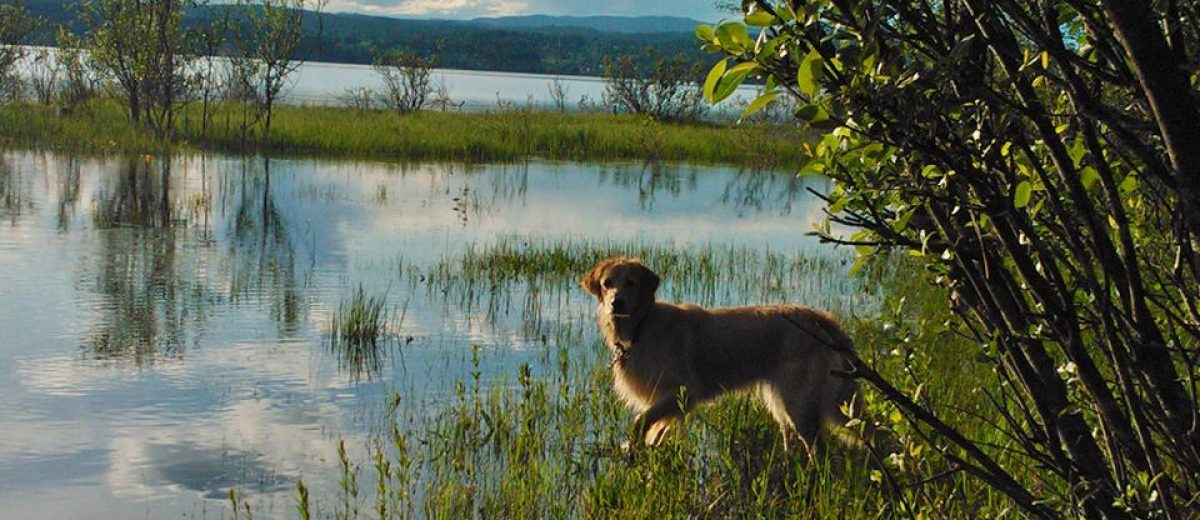
\includegraphics{fig/zelda.jpg}

\hypertarget{start-level-1}{%
\chapter{Start Level 1}\label{start-level-1}}

\hypertarget{start-level-2}{%
\section{Start Level 2}\label{start-level-2}}

\hypertarget{start-level-3}{%
\subsection{Start Level 3}\label{start-level-3}}

\hypertarget{part-appendices}{%
\part{Appendices}\label{part-appendices}}

\hypertarget{appendix-appendices}{%
\appendix}


\hypertarget{about}{%
\chapter{About}\label{about}}

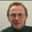
\includegraphics{fig/me.jpg}

\emph{Dyre Haugen} and \emph{Dyrehaugen} is Webian for \emph{Jon Martin} -
self-owned Globian, Webian, Norwegian and Canarian with
a background from industrial research policy, urban planning and
economic development consulting on global, regional and urban scales.
I am deeply concerned about the (insane) way
humanity (i.e.~capitalism) interfere with nature.
In an effort to gain insights in how and why this happens
stuff is collected from around the web and put together
in a linked set of web-sites.
The sites are operated as personal notebooks.
However, these days things can be easily published to the
benefit of others concerned with the same issues.
But be aware - this is not polished for presentation or
peer-reviewed for exactness.
I offer you just to have a look at my `work-desk' as it appears in the moment.
Any comment or suggestion can be mailed to \href{mailto:dyrehaugen@gmail.com}{\nolinkurl{dyrehaugen@gmail.com}}
You can follow me on twitter as @dyrehaugen.
Thanks for visiting!

\hypertarget{links}{%
\chapter{Links}\label{links}}

\textbf{Current Dyrehaugen Sites:}

\begin{itemize}
\tightlist
\item
  \href{https://dyrehaugen.github.io/rcap}{rcap - On Capitalism} \href{http://localhost/rcap}{(loc)}
\item
  \href{https://dyrehaugen.github.io/rclm}{rclm - On Climate Change} \href{http://localhost/rclm}{(loc)}
\item
  \href{https://dyrehaugen.github.io/recs}{recs - On Economics} \href{http://localhost/recs}{(loc)}
\item
  \href{https://dyrehaugen.github.io/rngy}{rfin - On Finance} \href{http://localhost/rfin}{(loc)}
\item
  \href{https://dyrehaugen.github.io/rngy}{rngy - On Energy} \href{http://localhost/rngy}{(loc)}
\item
  \href{https://dyrehaugen.github.io/renv}{renv - On Environment} \href{http://localhost/renv}{(loc)}
\item
  \href{https://dyrehaugen.github.io/rsts}{rsts - On Statistics} \href{http://localhost/rsts}{(loc)}
\item
  \href{https://dyrehaugen.github.io/rurb}{rurb - On Urbanization} \href{http://localhost/rurb}{(loc)}
\item
  \href{https://dyrehaugen.github.io/rvar}{rvar - On Varia} \href{http://localhost/rvar}{(loc)}
\item
  \href{https://dyrehaugen.github.io/rwsd}{rwsd - On Wisdom} \href{http://localhost/rwsd}{(loc)}
\end{itemize}

\textbf{Blogs:}

\begin{itemize}
\tightlist
\item
  \href{https://dyrehaugen.github.io/rde}{rde - Blog in English} \href{http://localhost/rde}{(loc)}
\item
  \href{https://dyrehaugen.github.io/rdn}{rdn - Blog in Norwegian} \href{http://localhost/rdn}{(loc)}
\end{itemize}

\textbf{Discontinued:}

\begin{itemize}
\tightlist
\item
  \href{https://dyrehaugen.github.io/jdt}{jdt - Collection (Jekyll)} \href{http://localhost/jdt}{(loc)}
\item
  \href{https://dyrehaugen.github.io/hdt}{hdt - Collection (Hugo)} \href{http://localhost/hdt}{(loc)}
\end{itemize}

\textbf{Not listed:}

\begin{itemize}
\tightlist
\item
  (q:) dhe dhn jrw56
\item
  (z:) rcsa rpad rstart
\end{itemize}

\hypertarget{news}{%
\chapter{NEWS}\label{news}}

  \bibliography{book.bib,packages.bib}

\end{document}
